\label{sec:exercise_install_go_env}

\subsection{Exercise M2GoEnvironmentInstallation}
\label{sec:exercise_m2go_environment_installation}

\subsubsection*{Environment Description}
The hardware used is a Windows Surface Studio with an 11th Gen Intel Core i5-11300H, 16 GB of RAM, and 256 GB of SSD storage.
The operating system is Windows 11 64-bit. However, the installation is carried out on WSL 2 running Ubuntu 20.04.6 LTS installed on the machine.

\subsubsection*{Installation Steps}
WSL2 (Ubuntu 20.04.6 LTS), VSCode (1.84.0) and Git (2.25.1) are already installed on the machine. Therefore no further installation steps are required for these tools.

Carrying out the installation of Go, version go1.21.3 is installed.
To install Go on the machine, the following steps are required:
\begin{enumerate}
    \item Download the latest version of Go from \url{https://go.dev/dl/go1.21.3.linux-386.tar.gz} by using  \texttt{wget}
    \item Extract the downloaded archive to \texttt{/usr/local} via \texttt{sudo tar -C /usr/local -xzf go1.21.3.linux-386.tar.gz}
    \item Under \texttt{/etc/profile} add the following lines to the bottom of the file: 
    \begin{itemize}
        \item \texttt{export PATH=\$PATH:/usr/local/go/bin}
        \item export \texttt{GOPATH=\$HOME/go}
    \end{itemize}
    \item Now reload the terminal or force the update by running \texttt{source \$HOME/.profile}
    \item Verify the installation by running \texttt{go version}
\end{enumerate}

\begin{figure}
	\centering
	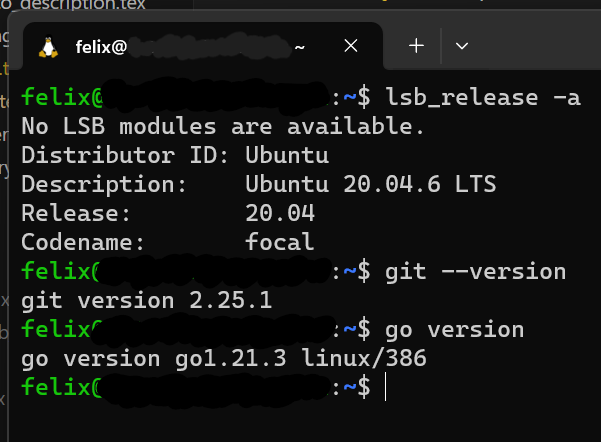
\includegraphics[width=0.8\textwidth]{figures/goLang/installation_screendump.png}
	\caption{Screendump showing the correct installation of the environment}
	\label{fig:screendump_installation}
\end{figure}

Further details on the installation and especially the path variables can be found in chapter \ref*{sec:go_environment_variables}.